\documentclass[11pt]{article}
\usepackage[margin=2cm,a4paper]{geometry}
\usepackage{graphicx}
\usepackage{amsmath}
\usepackage{amsfonts}
\usepackage{authblk}


\usepackage[superscript,biblabel]{cite}
\usepackage[super]{natbib}

\usepackage[style=numeric,sorting=none]{biblatex}
\addbibresource{references.bib}
\addbibresource{vancouver.bst}


\usepackage[outdir=./img/]{epstopdf}
\usepackage{epsfig}
\usepackage{url}
% Places figures at end of document, and do not print out the figures
\usepackage[nomarkers,nolists,tablesfirst]{endfloat}
%\renewcommand{\includegraphics}[2][]{}

\usepackage{xr}
\externaldocument{supplement}

\usepackage{tikz}
\usetikzlibrary{fit,positioning}
\usetikzlibrary{arrows}

\setlength\parindent{0pt}


\title{Illustrating Pathway activities with Sunburst plots}

\author[1]{The Authors}

\affil[1]{Science for Life Laboratory, KTH -- Royal Institute of Technology, Box 1031, 17121 Solna, Sweden\\
 Correspondence and requests for materials should be addressed to L.K. \\
 (email: lukas.kall@scilifelab.se)}


\begin{document}

\maketitle


\begin{abstract}

\end{abstract}

\section*{Introduction}
  Pathway analysis is a relatively new concept in biology, with publications increasing drastically in the last 10 years. Thanks to advances in computational power and databases, pathway analysis has become increasingly feasable as a way of data analysis. The greatest advantage of pathway analysis is that it lets us consider biological processes as units rather than each individual gene or protein. Using pathway databases like the reactome database \cite{reactome}, you can also look at the pathway hierarchy to define subprocesses of particular mechanisms.

  A common conundrum in biology is the observation that nothing occurs in isolation, for example, a ligand binding to a receptor does not only cause a conformational change in the receptor, but also leads to a plethora of secondary actions, all dependent on each other. To account for this potential Whac-a-mole when influencing a specific target it is a good idea to look at the target in its pathway context.

  A common practice in pathway analysis is to tabularly present results. While this does outline the most interesting pathways, a lot of information is lost to truncation. Furthermore, tabular presentations of pathway analysis seldomly characterize the hierarchical relationships of the pathways and even less so in a comprehensive manner.

  EnrichmentMap \cite{enrichmentmap}, a network-based method for pathway visualization uses network nodes and edges to display pathway gene overlap. While effective, it could lead to difficulties in interpretation when it comes to larger pathways with whom many pathways share genes. Therefore, a new way of pathway visualization has been proposed, sunburst plotting. Sunburst plotting uses the same idea of network nodes and edges, but implemented in a hierarchical manner.

  Considering the pathway hierarchy as a tree, with the largest pathways at the bottom, and each subprocess building on top, a sunburst plot simply rotates the tree around the origo to maximize visibility. This directed network significantly lowers the complexity of the undirected network seen in EnrichmentMap. This is partly due to the conceding that a pathway can exist in multiple pathway hierarchies, and the sunburst implementation thus incorporates the pathway at each of its hierarchical positions. To show the differences in pathway activities, we suggest the use of colors based on p-values or q-values.

  As an example, sunburst plotting with a color scale going from green to red as p-value decreases would in a comparison of samples that differ greatly in apoptosis see a red line in the apoptosis hierarchy.

  Sunburst plotting complemented by a tabular view of the most interesting pathways gives a better understanding of the cell. It incorporates hierarchial relationships as well as the complete picture of the cell landscape.


\section*{Methods}
  Skin cell scRNA-seq data from a single cell study on drug-induced hypersensitivity syndrome was analysed through iDEA \cite{idea}. iDEA requires differential expression data as input, which was obtained through the zingeR-DESeq2 method for R \cite{deseq2}. Subsequently, iDEA was run using gene sets from the reactome database. iDEA was run according to the tutorial outlined in the documentation with the only difference being the $min\_precent\_annot$ parameter being set to $5E-5$ instead of $2.5E-3$. This was to allow smaller pathways to be considered in order to produce the complete pathway hierarchy in the sunburst plot.

  The resulting data were compiled into a hierarchical json file containing pathway name, p-value, number of genes and rank. The JSON data was subsequently displayed as a sunburst plot. One methodological choice was to display the plots in html format rather than to use existing pythonic methods. This choice was mainly due to the javascript library d3.js (\url{https://d3js.org/}) allowing for great interactivity and the ability to draw the plots as SVG vectors.

  The display also took the data from the json file and displayed the 40 pathways with the lowest p-value in a table to show where the most interesting areas were. This was done as a complement to the sunburst plot, to allow for pattern identification and to aid in the search for specific pathways, in particular the less visible ones.

  As outlined in the introduction, the sunburst plot is a visualization of a tree-shaped network. The tree is simply rotated around the middle to maximize visibility. The size of the nodes are relative to the size of the pathway and in comparison to all other pathway at the specific hierarchical level.

  When it comes to the color scale, seen in figure \ref{fig:color_scale}, it scales from p=1 to p=0 from green to red. The scale is logarithmic in order to better discern pathways with high p-value from pathways with low p-value.

  In order to reduce clutter and excessive information, the sunburst plot utilizes an information box, seen in the center of figures \ref{fig:full_sunburst} and \ref{fig:mop_specific}. The box contains the pathway name, number of genes, p-value and rank to give specific information about the pathway in question.

  \begin{figure}[t]
    \centering
    \tikzstyle{start} = [rectangle, rounded corners, minimum width=3cm, text width=12cm, minimum height=1.7cm, text centered, draw=black, fill=red!10]
    \tikzstyle{iDEA} = [rectangle, rounded corners, minimum width=3cm, text width=12cm, minimum height=1.7cm, text centered, draw=black, fill=red!20]
    \tikzstyle{JSON} = [rectangle, rounded corners, minimum width=3cm, text width=12cm, minimum height=1.7cm, text centered, draw=black, fill=red!30]
    \tikzstyle{sunburst} = [rectangle, rounded corners, minimum width=3cm, text width=12cm, minimum height=1.7cm, text centered, draw=black, fill=red!40]
    \tikzstyle{arrow} = [thick, ->, >=stealth]

    \begin{tikzpicture}
    \node (start) [start] {Differential expression analysis};
    \node (iDEA) [iDEA, below of=start, yshift=-1.2cm]{Pathway analysis using the iDEA method};
    \node (JSON) [JSON, below of=iDEA, yshift=-1.2cm] {Generate hierarchical data structure including pathway information for sunburst plotting};
    \node (sunburst) [sunburst, below of=JSON, yshift=-1.2cm] {Sunburst plotting};

    \draw [arrow] (start) -- (iDEA);
    \draw [arrow] (iDEA) -- (JSON);
    \draw [arrow] (JSON) -- (sunburst);

    \end{tikzpicture}
  \caption{ A flowchart representation of the pipeline developed for this article.}
  \label{Pipeline flowchart}
\end{figure}

\subsection*{Datasets}
  Datasets are available at \url{https://www.ncbi.nlm.nih.gov/geo/query/acc.cgi?acc=GSE132802}
\subsection*{Code availability}
  Code is available at \url{https://github.com/statisticalbiotechnology/porch}

\section*{Results}

  Results from the iDEA pathway analysis of the single cell data can be seen in figure \ref{fig:full_sunburst} with the color scale in figure \ref{fig:color_scale}. At first glance, you can already tell where the focal points of the study lie. If you consider the plot like a clock, around one o'clock, the pathway with the lowest p-value, metabolism of proteins \cite{reactome} lies. Translation, a child pathway of metabolism of proteins, can be seen in orange right above. Around eight o'clock, the metabolism pathway can be found.

  Also seen in the middle of \ref{fig:full_sunburst} is a box containing information on the pathway at hand. Perhaps not demonstrated perfectly in a static image, the box follows the computer mouse and displays information over which pathway the mouse hovers. The greatest advantage of this is to display the name of the pathway in question, however, information on the number of genes and p-value can definitely come in handy, especially in cases where the pathway can't be found in the table.

  Clicking a specific pathway can be used as a zooming tool. Seen in figure \ref{fig:mop_specific} is the sunburst specific for the metabolism of protein pathway. This plot has the same logic as the full sunburst, with every outer circle being one step further from the main pathway in question. Since the reactome database contains around 2000 pathways, a way of displaying them all would have to find a way of fitting them all into a neat container. The interactive step of being able to view specific pathways individually solves this, by producing a new canvas independent of the complete pathway hierarchy. To aid in navigation, a navigation bar of the pathway hierarchy can be used.

  As can be seen in figure \ref{fig:full_sunburst}, this was done by sizing the cells by pathway size. The middle being

  Furthermore, one quick observation is that the iDEA pathway analysis method seem to prefer larger pathways as the larger pathways tended to be colored more orange, whilst smaller pathways tended to be more green.

  GSEA BRCA analysis.

  The use of sunburst plots has also been demonstrated in cancer transcriptomics. The large metabric dataset for breast cancer was analysed through GSEA, comparing a number of different groups. An example comparing BRCA1 mut/WT samples can be seen figure \ref{fig:brca1}. Compared to the single cell example, GSEA gives clearer "lines" of parent/child pathways following the same pattern. This





\begin{figure}[htp]
\begin{center}
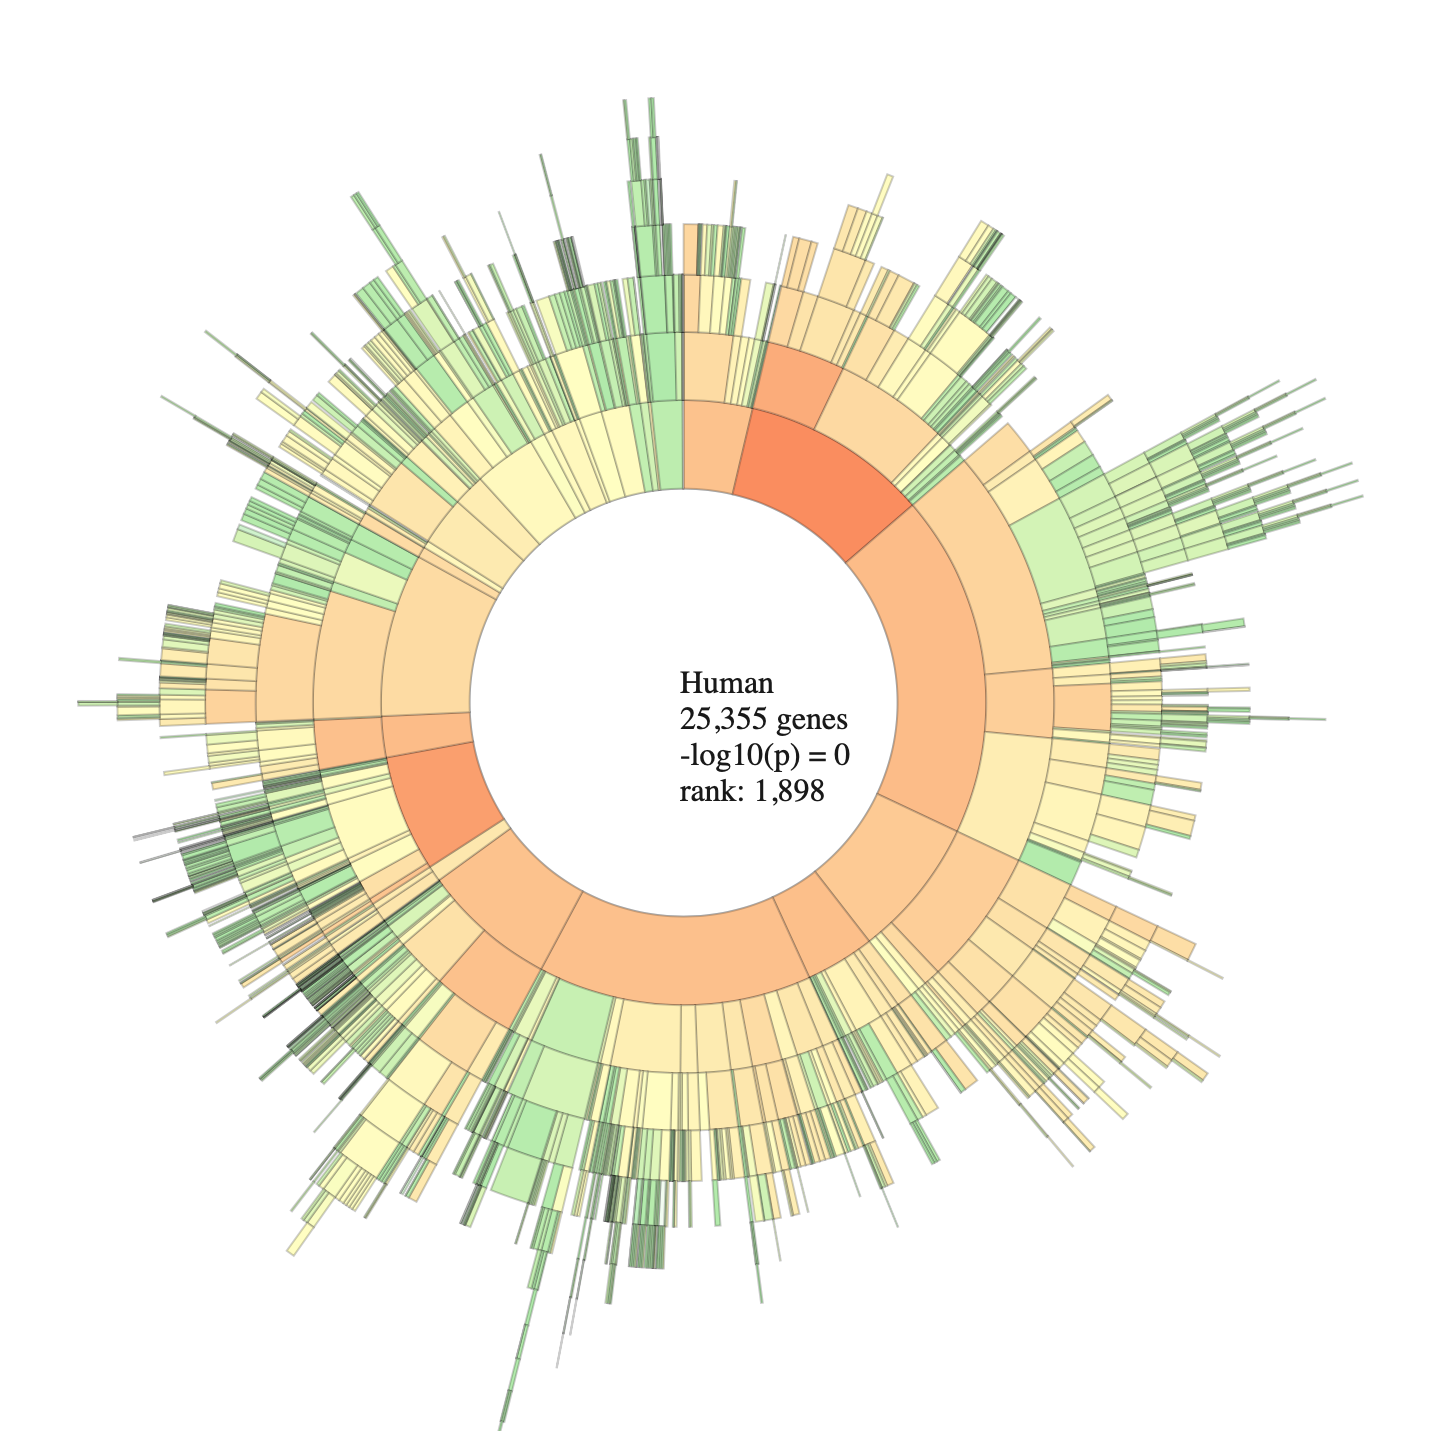
\includegraphics[width=0.96\linewidth,clip]{./img/full_sunburst.png}
\caption{\label{fig:full_sunburst} {\bf Sunburst plot.} Hierarchical representation of all cellular pathways colored by p-value}
\end{center}
\end{figure}

\begin{figure}[htp]
\begin{center}
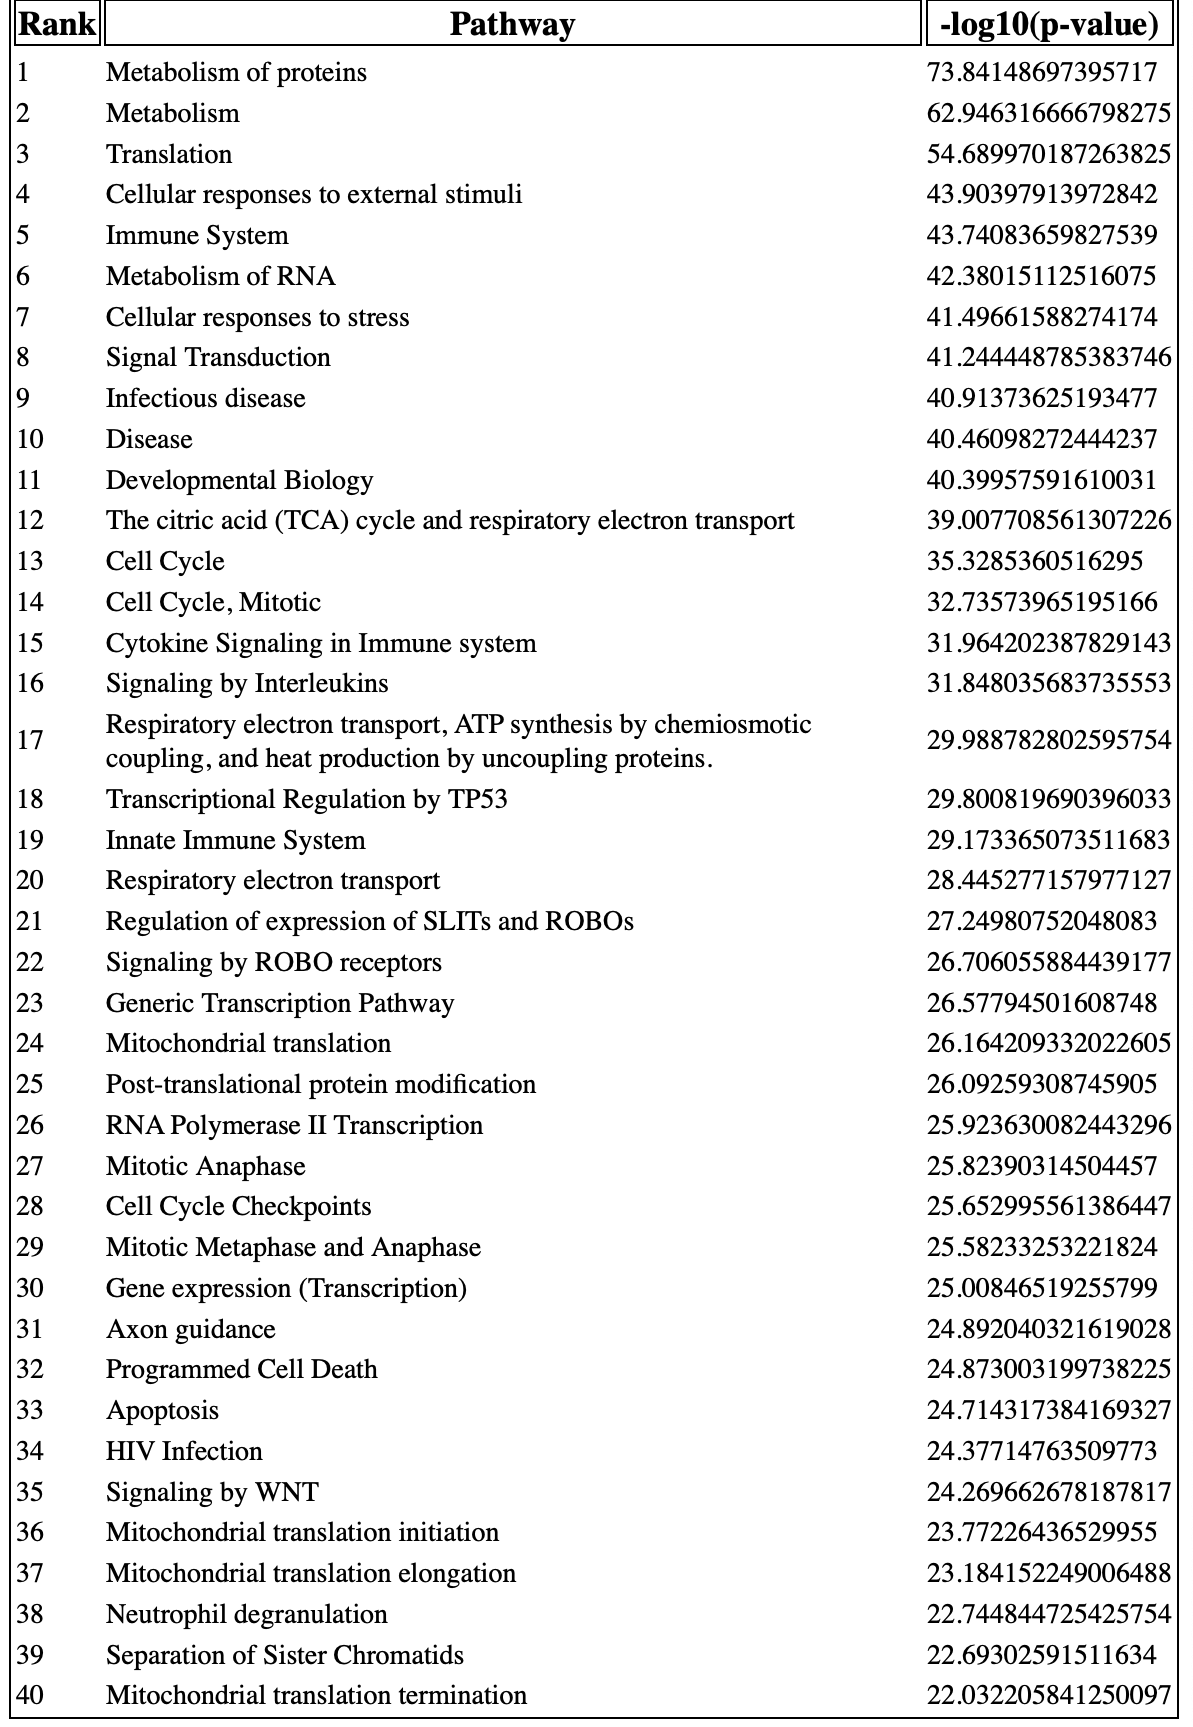
\includegraphics[width=0.96\linewidth,clip]{./img/table.png}
\caption{\label{fig:table} {\bf Pathway table.} Tabular representation of the 40 pathways with the lowest p-value}
\end{center}
\end{figure}

\begin{figure}[htp]
\begin{center}
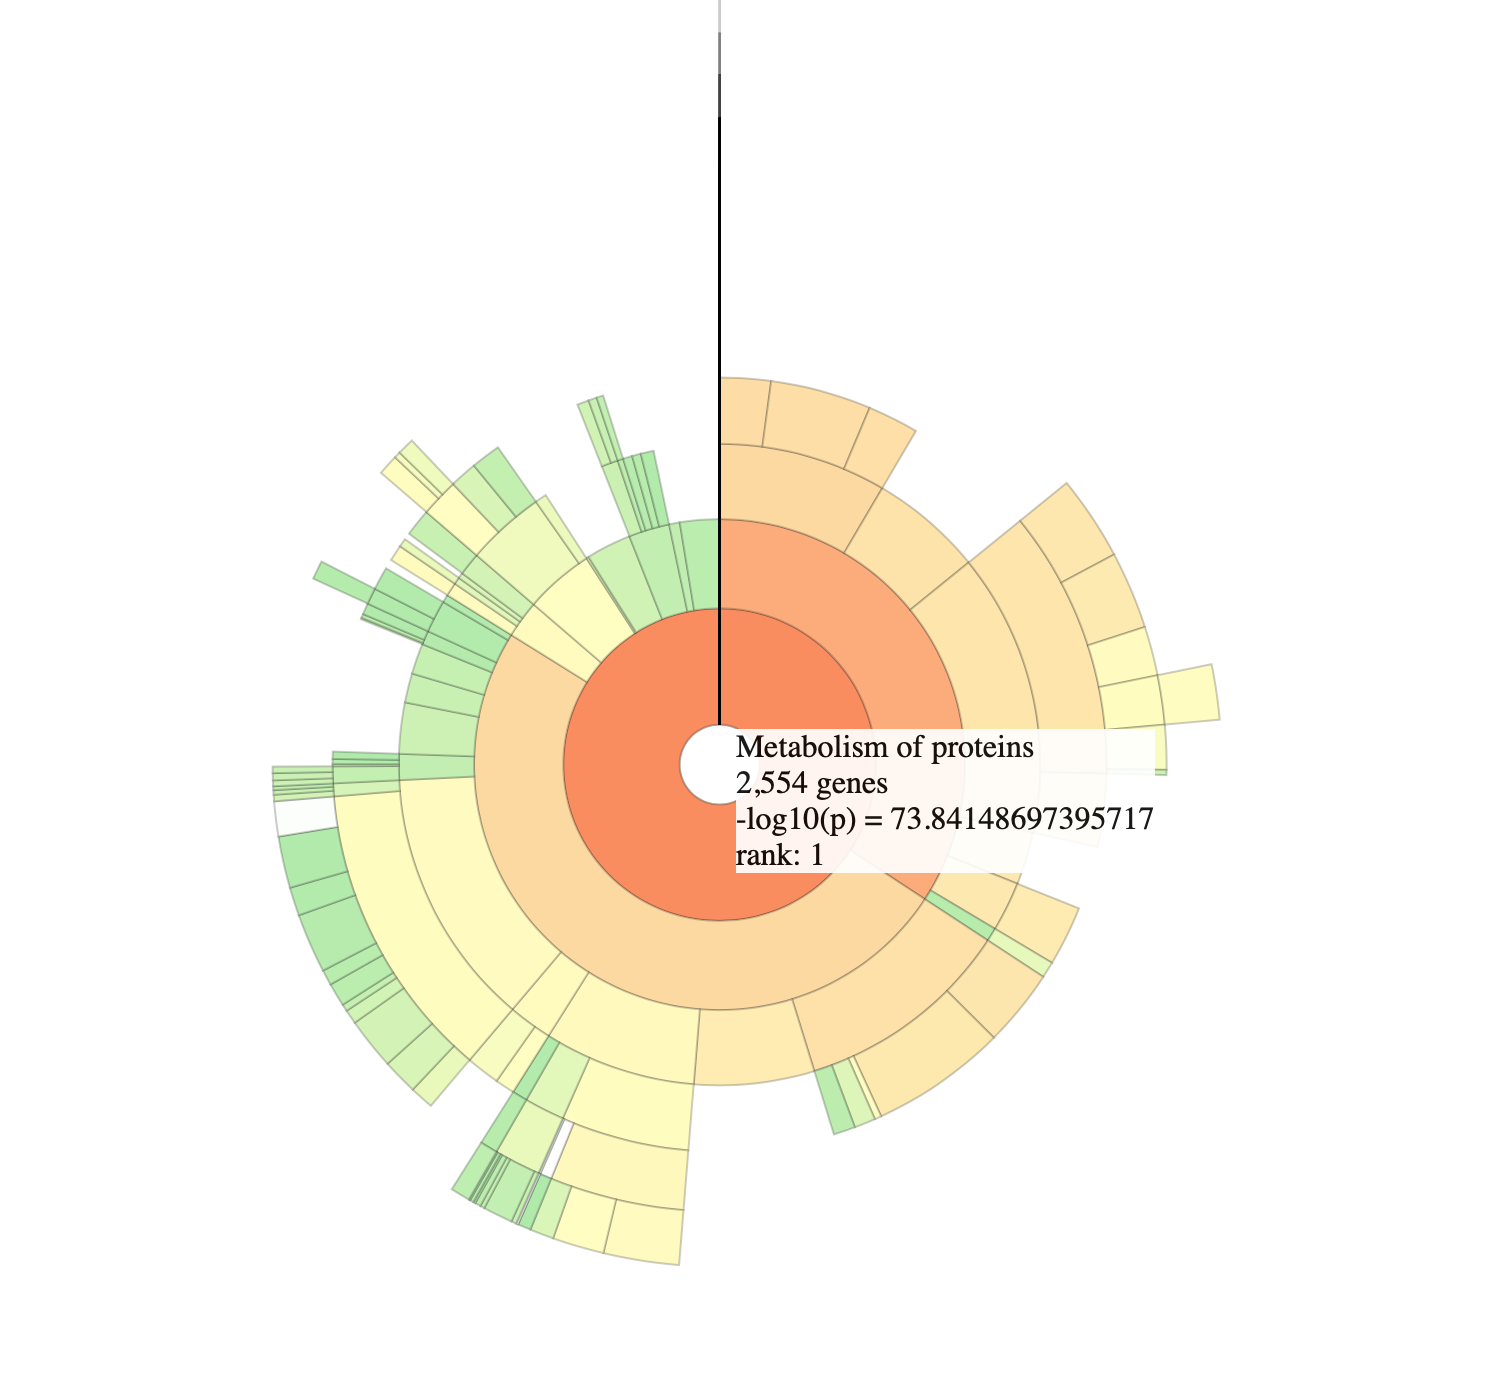
\includegraphics[width=0.96\linewidth,clip]{./img/mop_specific.png}
\caption{\label{fig:mop_specific} {\bf Pathway specific sunburst.} Sunburst plot drawn specifically for the metabolism of proteins pathway hierarchy}
\end{center}
\end{figure}

\begin{figure}[htp]
\begin{center}

\includegraphics[width=0.96\linewidth,clip]{./img/color_scale.png}
\caption{\label{fig:color_scale} {\bf Sunburst color scale.} The sunburst color scale annotated by which p-value they represent.}
\end{center}
\end{figure}

\begin{figure}[htp]
\begin{center}
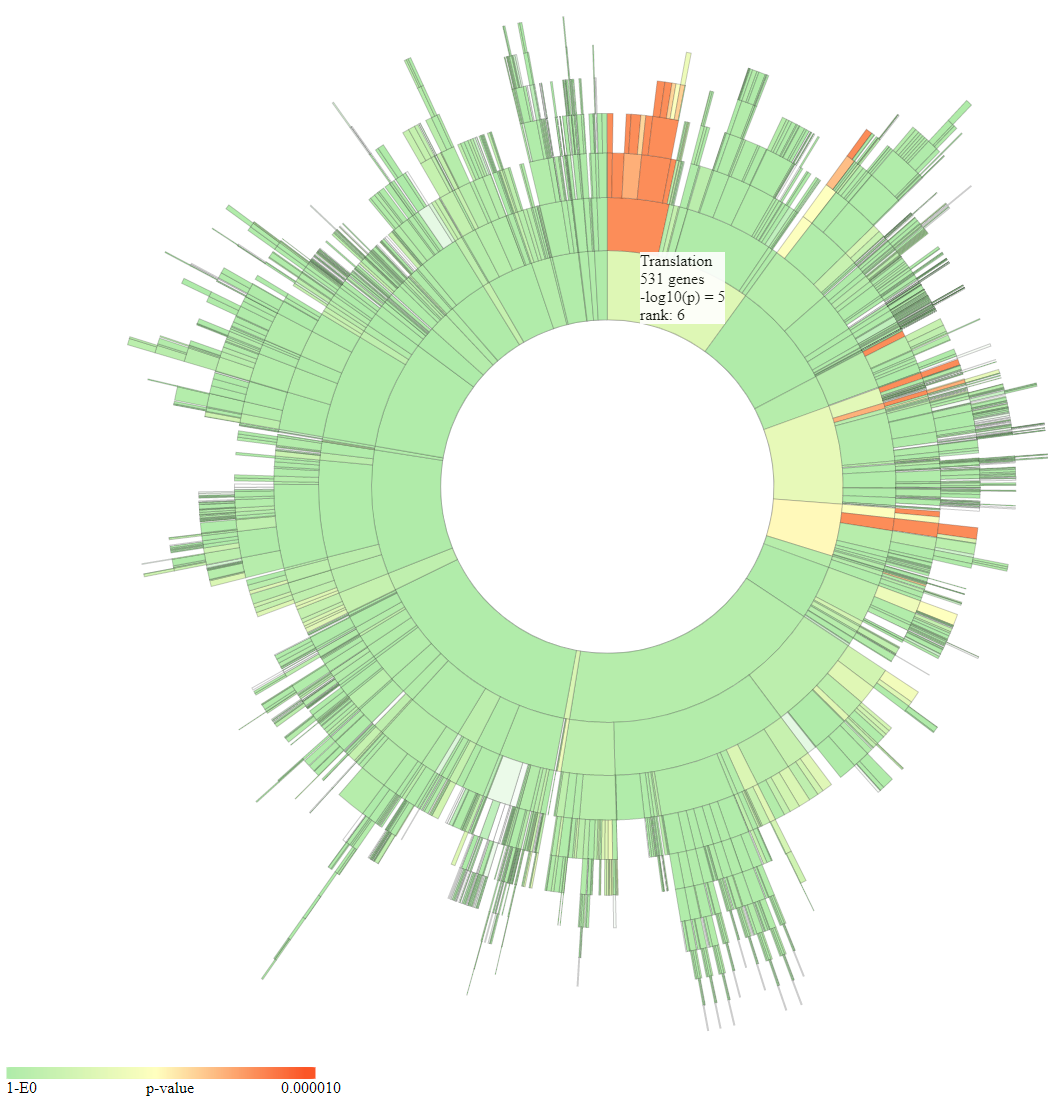
\includegraphics[width=0.96\linewidth,clip]{./img/BRCA1.png}
\caption{\label{fig:brca1} {\bf Metabric GSEA} A sunburst representation of GSEA comparing BRCA1 mut/WT.}
\end{center}
\end{figure}

\section*{Discussion}
  One of the greatest advantages of sunburst plotting is the possibility to view all cellular pathways simultaneously in their hierarchical context. Tabular views generally only gives a glimpse of the most interesting pathways while neglecting the bulk of pathways.

  Sunburst plotting as a complement to a tabular view gives a more holistic view of pathway activities in the cell.

  One great feature of sunburst plots is the possibility to see parent-child pathway relationships. As seen in figure \ref{fig:mop_specific}, child-pathways of the metabolism of proteins pathway have quite different p-values.

  Another advantage of sunburst plotting is the speed to which a primary conclusion can be made of where the focal points of the experiment lie. While tables might give a similar conclusion, a significant amount of time will have to be spent to reach it.

  Sunburst plotting together with the tabular analysis described above became an excellent combination of analyses as the table provides very specific information of the pathways and the sunburst plots provide a broader picture of the pathway relationships of cells.

  One aspect where the advantage of using sunburst plotting became undeniable was when analysing parent child pathway relationships. As can be seen in figure \ref{fig:mop_specific}, the expression of some pathways (green) differs from the activity of Z (orange). This thus becomes somewhat of a barcoding analysis where a straight line of parent child pathways with low p-value is quite convincing evidence against type I errors.

  Seeing as this is a relatively novel method of analysis, a few points of benchmarking and what the underlying biology might be have been developed.

  \begin{itemize}
      \item A parent pathway with relatively medium p-value and several child-pathways where at least one of them has very low p-value is a good indicator that the parent pathway p-value might be affected by a change in the significant child pathway.
      \item A significant pathway with no children should be an interesting pathway to study as it has been broken down as much as possible and still poses a significant difference in activity compared to other clusters.
      \item A significant parent pathway with insignificant child pathways need to be examined further as neither of the subprocesses have been deemed significant.
    \end{itemize}

\section*{Acknowledgments}

This work was supported by a grant from the Swedish Research Council (grant
2017-04030).

\section*{Author Contributions}

\section*{Competing interests}

The authors declare that they have no conflict of interest.

\printbibliography[title=References]

\end{document}
